% !TeX program = xelatex
% MetaCircle arXiv source. Build with: latexmk -xelatex main.tex
\documentclass[11pt]{article}
\usepackage[round,authoryear]{natbib}
\PassOptionsToPackage{no-math}{fontspec}
\usepackage{metacircle}
\usepackage{float}
\usepackage{array}
\usepackage{multirow}

\renewcommand{\topfraction}{0.95}
\renewcommand{\bottomfraction}{0.5}
\renewcommand{\textfraction}{0.05}
\renewcommand{\floatpagefraction}{0.8}
\graphicspath{{figures/}}

\newcommand{\KL}{\operatorname{KL}}
\newcommand{\Var}{\operatorname{Var}}
\newcommand{\E}{\mathbb{E}}
\newcommand{\RMS}{\operatorname{RMS}}
\newcommand{\q}{q}
\newcommand{\p}{p}
\newcommand{\pt}{p_t}
\newcommand{\pzero}{p_0}

\title{Beyond Relative Generalization Invariance: Shared Difficulty and Local Learning Response\\in Language Model Training}
\author{
  Shaoyang Guo$^{*}$ and Ziming Liu$^{*,\dagger}$\\
  \small $^*$Core contributors, equal contribution \quad $^\dagger$Corresponding author
}
\date{}
\paperdate{October 6, 2026}
\papertype{Meta Circle Research}
\projecturl{}

\begin{document}
\maketitle

\begin{metaabstract}
We study what is shared, and what is optimizer-dependent, in teacher-forced language-model loss.  The recent Relative Generalization Invariance (RGI) result reports that token-wise loss differences can remain highly similar across training choices, but it does not identify the finite-update terms responsible for a Transformer trajectory.  We decompose an arriving-batch loss into a frozen-data difficulty and a local response.  For an update from \(\theta_0\) to \(\theta_t\), the response has an exact linear-work term \(A=\nabla_\theta\ell(\theta_0)^\top(\theta_t-\theta_0)\), a nonnegative logit-space curvature term \(Q=\operatorname{KL}(p_0\Vert p_t)\), and a representation residual.  Its second-order logit approximation is \(A+Q_2\), with \(Q_2=\tfrac12\operatorname{Var}_{p_0}(\Delta z)\).

Across three permutations of a fixed FineWeb pool and SGD or Adam continuation of Pythia-70M, a common step-32,000 reference explains 96.657--97.582\% of arriving-loss variance; each algorithm's frozen start explains 99.940--99.997\% in the registered near and far windows.  On the residual slow signal \(L-D\), observed-displacement \(A+Q_2\) has 4.97--9.73\% relative RMS error for SGD and 1.19--2.82\% for Adam, with at least 96.87\% variance explained.  Signed covariance shows negative linear work and positive curvature cancel, and both terms change with the optimizer.  A single scalar probe does not close the batch-specific response, and the optimizer difference fails the 10\% response gate.  A fixed-teacher continuation closes the same local decomposition, but its cross-prefix optimizer gap still fails a strict constant-offset test.  We therefore obtain a quantitative local finite-displacement mechanism and a clear boundary: the evidence does not establish a universal strong-RGI mechanism for natural language models.

\keywords{language model training, teacher forcing, optimization dynamics, relative generalization invariance, cross-entropy}
\end{metaabstract}

\section{Introduction}

The loss of a language model mixes two sources of variation that are usually reported together.  A batch can be intrinsically difficult under a fixed predictor, while the predictor can also move during training.  The first source changes when the next batch changes; the second accumulates through the optimizer and the model's local geometry.  A useful explanation of training loss should identify these terms on the same teacher-forced targets and should say which term dominates at the scale being measured.

Zhang et al.~\citep{zhang2026relativegeneralizationinvariancellm} introduced Relative Generalization Invariance (RGI): the validation-loss difference between two models is approximately preserved across tokens.  Their experiments show strong empirical similarity across optimizers and moderate architectural changes, while their quadratic example gives a sufficient stylized construction.  The result leaves open a more local question: when a real Transformer receives one arriving batch, which terms create the common fast variation, and which terms create the slower optimizer-dependent response?  This distinction matters because high correlation of two loss curves does not imply a constant token-wise gap.

We test the following concrete version of the question.  Let \(D(B)\) be the teacher-forced cross-entropy of a fixed start model on batch \(B\), let \(L_t(B)\) be the same score after an observed continuation, and write \(M_t(B)=L_t(B)-D(B)\).  We ask whether \(D\) explains the large batch-to-batch variation, and whether \(M\) is explained by a frozen gradient acting on the observed parameter displacement plus softmax curvature.  We do not fit a slope or intercept on the evaluation window, and we do not treat an identity using the final logits as a forecast of an unknown future update.

Our contributions are:
\begin{itemize}
  \item We give a teacher-forced, batch-level decomposition that separates frozen difficulty from finite local response and measures each term directly.
  \item In a registered Pythia-70M continuation, a common frozen reference explains 96.657--97.582\% of raw arriving-loss variance, while the algorithm-specific frozen starts explain at least 99.940\% in the far window.
  \item On the slow signal itself, \(A+Q_2\) closes all six natural near, far, and full windows at the registered 10\% RMS and 90\% variance thresholds.  The signed terms show that linear learning gain and positive curvature cost both matter.
  \item We document the boundary of this explanation: a scalar global probe is insufficient, the optimizer-difference response fails the 10\% gate, and a known-teacher population test does not yield a constant token-wise optimizer offset.
\end{itemize}

The claims are deliberately local.  We study finite Pythia-70M continuations with reset optimizer state, not a reproduction of the original paper's 124M and 0.7B pretraining runs.  The main conclusion is a measured response mechanism for these trajectories, together with a substantive obstruction to promoting it to a universal explanation of strong RGI.

\section{Relation to RGI and scope of the claim}

RGI compares a pair of models on the same teacher-forced target and asks whether their loss difference is approximately independent of the token.  We retain that paired evaluation, but separate two notions that are easy to conflate.  A weak statement is that two loss vectors have high correlation or a small relative-difference statistic.  A strong statement is that
\begin{equation}
  \ell_A(x,y)-\ell_B(x,y) \approx c
  \quad\text{for every evaluated prefix--target pair,}
  \label{eq:strong-rgi}
\end{equation}
with a residual small relative to \(|c|\).  The latter is the constant-offset mechanism that would make the optimizer choice nearly irrelevant to token ranking.

Our experiment is designed to locate terms before testing Eq.~\eqref{eq:strong-rgi}.  On a natural target, an arbitrary checkpoint reference \(q\) is not the unknown conditional data distribution.  Therefore a reference KL is a measurable comparison to \(q\), not a natural Bayes excess risk.  For a fixed teacher distribution we can remove this ambiguity, but that changes the task to a known-teacher continuation.  We report the two settings separately.

The prior quadratic construction is a sufficient example in a different model class.  It does not by itself identify the representation term or optimizer response of a Transformer.  Our evidence likewise does not claim that natural LLMs satisfy the sufficient conditions of that construction.  Instead, it tests whether the more concrete finite-displacement terms below account for the observed slow response and then checks whether the remaining paired gap is actually constant.

\section{A finite-update decomposition}

Consider one prefix--target pair \((x,y)\), with logits \(z_0(x)\) at the frozen start \(\theta_0\), probabilities \(p_0=\operatorname{softmax}(z_0)\), and logits \(z_t\) after the observed continuation.  Write \(\Delta z=z_t-z_0\), \(p_t=\operatorname{softmax}(z_t)\), and \(e_y\) for the one-hot target.  For a batch, all quantities below are averaged over the same target positions.

The frozen difficulty is
\begin{equation}
  D(B)=\operatorname{mean}_{(x,y)\in B}\left[-\log p_0(y\mid x)\right].
  \label{eq:difficulty}
\end{equation}
The exact change in cross-entropy has a useful logit-space identity,
\begin{align}
  L_t(B)-D(B)&=W(B)+Q(B),\\
  W(B)&=\operatorname{mean}\left[(p_0-e_y)^\top\Delta z\right],\\
  Q(B)&=\operatorname{mean}\left[\KL(p_0\Vert p_t)\right]\geq 0.
  \label{eq:exact}
\end{align}
The equality follows from the log-partition identity and is used as an arithmetic check.  It is not a forecast because it uses the observed final logits.

To connect the loss change to parameter motion, recompute the batch gradient at \(\theta_0\) and define
\begin{equation}
  A(B)=\nabla_\theta\ell_{\theta_0}(B)^\top(\theta_t-\theta_0),
  \qquad R(B)=W(B)-A(B).
  \label{eq:work}
\end{equation}
The exact change can then be written \(L_t-D=A+R+Q\).  The residual \(R\) includes the nonlinearity of the parameter-to-logit map along the observed displacement, as well as any replay or numerical error; we do not identify it with a single unmeasured Hessian term.

The second-order logit approximation to the convex log-partition term is
\begin{equation}
  Q_2(B)=\frac12\operatorname{mean}_{(x,y)\in B}\left[\operatorname{Var}_{v\sim p_0(\cdot\mid x)}\left(\Delta z_v(x)\right)\right].
  \label{eq:q2}
\end{equation}
Our primary local closure is therefore \(L_t-D\approx A+Q_2\).  Both \(A\) and \(Q_2\) use the displacement that actually occurred: \(A\) uses \(\theta_t-\theta_0\), and \(Q_2\) uses \(\Delta z\).  The test explains a realized finite response; it does not predict a future response from a frozen gradient alone.

For a fixed teacher distribution \(q(\cdot\mid x)\), the same algebra replaces \(e_y\) by \(q\).  With \(p_t=\operatorname{softmax}(z_q+v)\), the teacher-forced hard-target loss decomposes as
\begin{equation}
  \ell=S+C+E,\qquad S=-\log q_y,\quad C=(q-e_y)^\top v,\quad E=\KL(q\Vert p_t).
  \label{eq:teacher}
\end{equation}
Under a target drawn from \(q\), \(\mathbb{E}_q[C\mid x]=0\), and the population cross-entropy is \(H(q)+E\).  We use this controlled population objective to separate label sampling from the natural-text case, where the unknown conditional distribution is not observed.

\section{Experimental protocol}

\paragraph{Natural continuation.}
We use the public Pythia-70M architecture~\citep{biderman2023pythiasuiteanalyzinglarge} and official step-32,000 checkpoint as the shared reference and continue the model locally.  The model has 70,426,624 trainable parameters and the verified Pythia tokenizer has vocabulary size 50,304.  The new data pool contains 4,672 length-qualified FineWeb sample-10BT documents~\citep{penedo2024finewebdatasetsdecantingweb} from revision \texttt{9bb295dd...}, with source rows beginning at 65,536.  We select one random 256-token span per document, exclude registered prior IDs, text hashes, and exact spans, and split 4,096/64/512 documents into training, calibration, and evaluation pools.  Selection used no model score.  The data source is not claimed to be absent from Pythia pretraining or to be domain extrapolation.

Three fixed permutations of the same pool are run for 512 updates with batch size 8 and context length 256.  The continuation starts from the corresponding completed SGD or Adam trajectory and resets optimizer state.  SGD uses learning rate \(10^{-3}\); Adam~\citep{kingma2017adammethodstochasticoptimization} uses learning rate \(10^{-6}\), betas \((0.9,0.95)\), and \(\epsilon=10^{-8}\).  These are controlled local continuations, not the historical Pythia AdamW/Pile pretraining process.  The common frozen reference \(q\) is the official step-32,000 model; each algorithm also has its own frozen start \(p_0\).

\paragraph{Known teacher.}
The teacher is the official step-32,000 model.  From 33-token natural seeds, it samples 63 autoregressive tokens at temperature one using the full 50,304-token vocabulary.  The resulting 1,216 documents are split 1,024/64/128 for training, calibration, and evaluation.  A student starts from official step 16,000 and trains for 128 updates under either hard sampled targets or the full soft teacher distribution~\citep{hinton2015distillingknowledgeneuralnetwork}, with the same three permutations and two optimizers.  This is a synthetic known-teacher conditional task, not an estimate of the natural Bayes distribution.

\paragraph{Readouts and gates.}
For each arriving batch we record teacher-forced \(L_t\), frozen \(D\), \(A\), \(W\), \(Q\), \(Q_2\), and \(R\).  We predeclare near \(0{:}128\), far \(384{:}512\), and full \(0{:}512\) windows.  Relative RMS error and variance explained \(1-\operatorname{MSE}/\operatorname{Var}\) are reported separately.  The primary gates are 10\% relative RMS and 90\% variance explained.  We also report 64-step block means, high-pass residuals, and signed covariance shares \(\operatorname{Cov}(M,T)/\operatorname{Var}(M)\), which can be negative and sum to one.

The frozen-difficulty windows were registered before the fresh continuation.  The arrival-batch and logit-work analyses are retrospective diagnostics of completed trajectories.  Independent verifiers checked saved traces, hashes, identities, and fixtures; they did not independently recompute the full network gradients or the complete parameter trajectories.

\section{Frozen difficulty explains the fast variation}

The first question is whether the large variation of arriving-batch loss is already present in a model that is not updated.  Figure~\ref{fig:numerical-theory}a compares each arriving loss with the score from the corresponding frozen start, without fitting an offset or slope.  Across the three permutations and two algorithms, the frozen start explains 99.9943--99.9974\% of near-window variance and 99.9400--99.9713\% of far-window variance.  The frozen-start RMSE is 0.000916--0.001330 nats near and 0.003663--0.004736 nats far.  The standard deviation of \(D\) is 0.1761--0.2165 nats, much larger than the slow response.

To test whether this is an artifact of choosing a separate reference for each optimizer, we use the single official step-32,000 reference \(q\) for both trajectories.  It explains 96.657--97.578\% of near-window variance and 96.745--97.582\% of far-window variance.  Thus the shared data term remains the dominant source of raw loss variation even under a common reference.

This result is a scale statement, not an independence theorem.  If \(\sigma_D=\operatorname{std}(D)\), \(m=\RMS(M)\), and \(\rho=m/\sigma_D<1\), the reverse triangle inequality gives
\begin{equation}
  1-\frac{\operatorname{MSE}(L,D)}{\operatorname{Var}(L)}
  \geq 1-\left(\frac{\rho}{1-\rho}\right)^2.
  \label{eq:scale-bound}
\end{equation}
The observed far-window \(\rho\) is at most 0.024482, which alone gives a conservative 99.937\% lower bound.  The bound does not say that difficulty and response are statistically independent, and it only applies to teacher-forced targets whose labels are already known.

\begin{figure}[t]
  \centering
  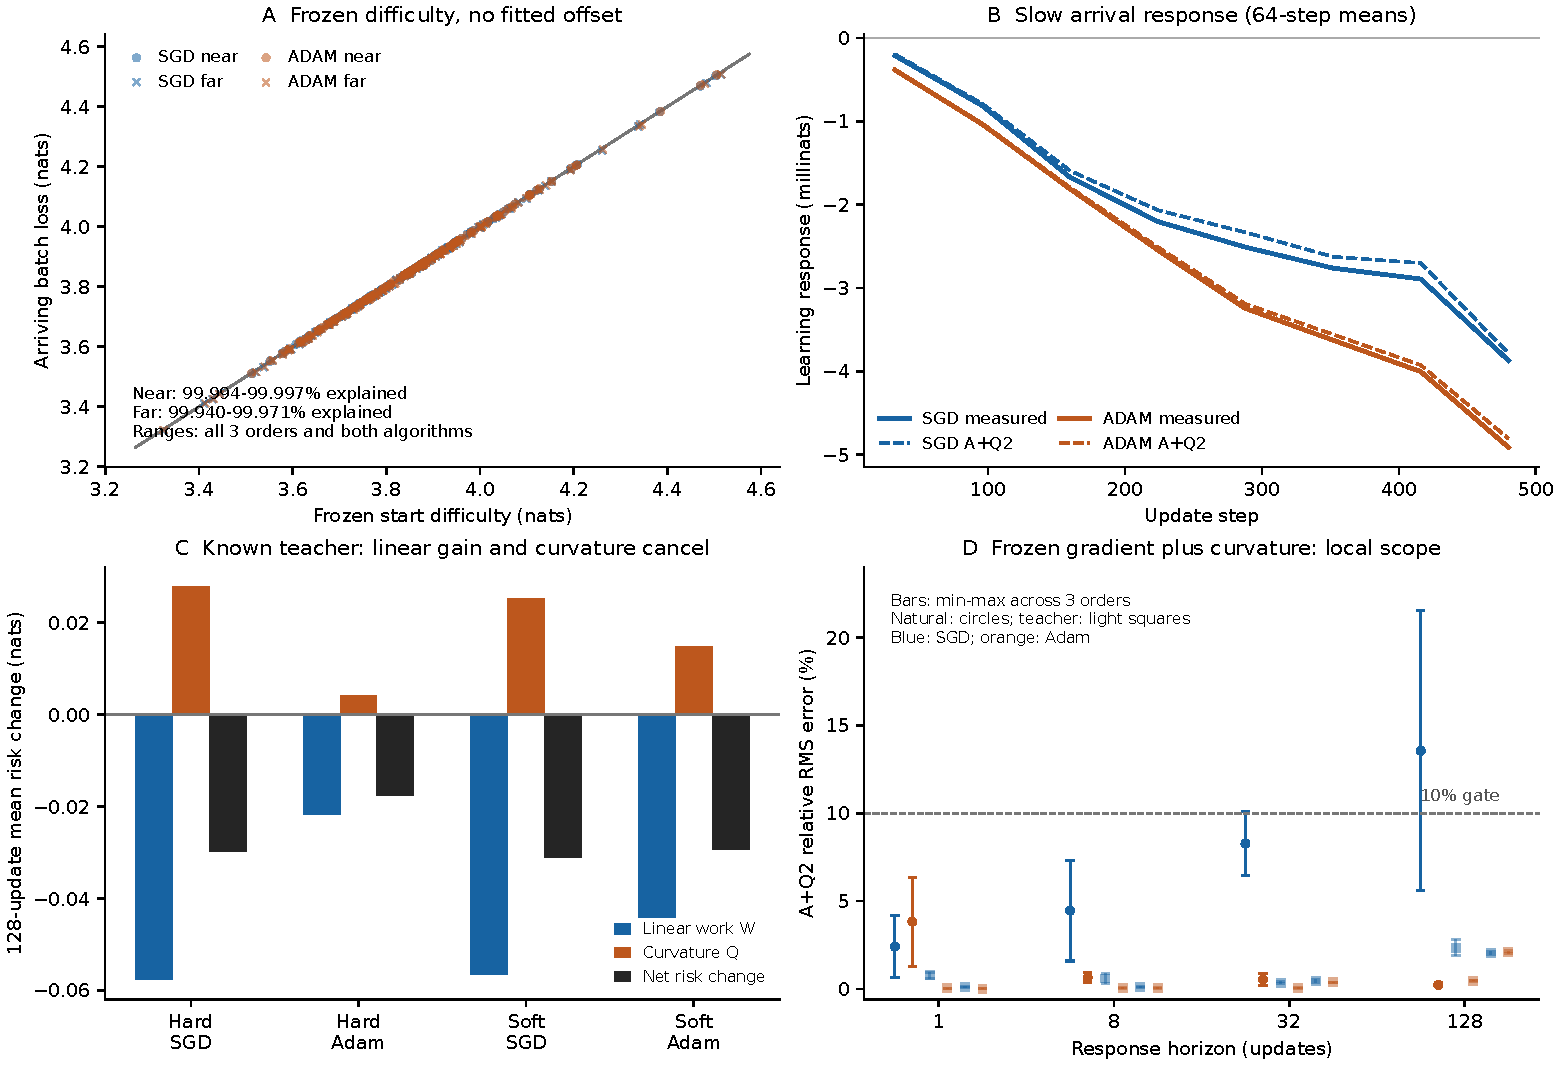
\includegraphics[width=\linewidth]{numerical-theory.pdf}
  \caption{Four views of the measured decomposition.  (a) Frozen start difficulty versus arriving loss.  (b) Measured slow response and the observed-displacement \(A+Q_2\) closure.  (c) In the known-teacher task, negative linear work and positive curvature cancel.  (d) Local closure error across response horizons.  Ranges and gates are summarized in the text; the plotted trajectories are finite measurements, not confidence intervals.}
  \label{fig:numerical-theory}
\end{figure}

\section{What closes the slow response?}

Table~\ref{tab:arrival} reports the primary arrival-batch test on \(M=L-D\), rather than hiding the response under the much larger variance of \(L\).  All six natural trajectories pass both gates in all three windows.  SGD has 4.97--9.73\% relative RMS error and 96.87--99.71\% explained variance; Adam has 1.19--2.82\% and 99.27--99.96\%, respectively.  The result is strongest for Adam and remains within the predeclared RMS gate for SGD in the far window.

\begin{table}[t]
\centering
\caption{Relative RMS error and variance explained for \(A+Q_2\) on the slow response \(L-D\).  Each range spans three permutations.}
\label{tab:arrival}
\small
\begin{tabular}{llcc|cc}
\toprule
 & & \multicolumn{2}{c|}{SGD} & \multicolumn{2}{c}{Adam}\\
Window & signal & RMS & explained & RMS & explained\\
\midrule
Near & raw & 4.97--9.12\% & 98.95--99.71\% & 1.19--1.69\% & 99.924--99.963\%\\
Far & raw & 6.53--9.33\% & 96.87--98.55\% & 2.49--2.82\% & 99.273--99.377\%\\
Full & raw & 7.13--9.73\% & 98.04--98.98\% & 2.38--2.59\% & 99.780--99.799\%\\
\bottomrule
\end{tabular}
\end{table}

The term means identify the direction of the response.  Across full 512-step arrival batches, SGD has mean \(A=-0.004011\) to \(-0.003552\) nats, \(Q=+0.001740\) to \(+0.001981\), and \(L-D=-0.002153\) to \(-0.001892\).  Adam has \(A=-0.003290\) to \(-0.003272\), \(Q=+0.000609\) to \(+0.000621\), and \(L-D=-0.002699\) to \(-0.002690\).  On 64-step block means, the signed covariance shares of \(A\) are 1.51--1.62 for SGD and 1.25--1.26 for Adam, while the shares of \(Q\) are -0.66 to -0.54 and -0.28 to -0.27.  Negative work creates improvement; positive curvature cancels part of it.  The optimizer changes both terms.

The closure is local and has measurable failure modes.  After removing 64-step block means, SGD's high-pass relative RMS error is 10.75--16.68\% in the far window; the remaining error is mainly \(R=W-A\), while \(Q-Q_2\) is below 1\% of the response.  The optimizer-difference response, tested as \(\Delta A+\Delta Q_2\), has 10.34--16.68\% full-window error in all three replicas, despite 96.74--98.57\% variance explained.  Subtracting two small responses magnifies the representation residual.

\section{A global scalar probe is not enough}

An independent 64-document probe produces a scalar \(U(t)\).  It tracks the raw loss well because the frozen difficulty is large, but its relative RMS error on \(M\) is 45.1--90.0\% near, 29.5--55.2\% far, and 31.7--62.8\% over the full continuation.  Interpolating with the next checkpoint, which is a deliberately noncausal diagnostic, leaves 29.1--54.7\% far-window error.  The missing information is batch-specific sensitivity: \(A(B)\) uses the arriving batch's frozen gradient, whereas a single global score does not.

\section{Local response and optimizer terms}

The exact identity in Eq.~\eqref{eq:exact} is useful for checking arithmetic, but it does not assign causal responsibility.  The measured decomposition adds the frozen-gradient work \(A\) and the positive curvature approximation \(Q_2\).  On all six natural trajectories, \(A+Q_2\) passes the primary raw-window gates reported in Table~\ref{tab:arrival}.  The remaining error is not uniformly negligible: the SGD high-pass far-window test reaches 16.68\%, and the paired optimizer-difference test reaches 16.68\% at worst.  These failures are evidence that batch-specific representation response matters after the large common difficulty term is removed.

For the full arrival window, the mean residual \(R=W-A\) is \(-1.24\times10^{-4}\) to \(-0.81\times10^{-4}\) nats for SGD and \(-3.31\times10^{-5}\) to \(-2.98\times10^{-5}\) for Adam, with RMS 0.000189--0.000285 and 0.0000640--0.0000724, respectively.  The curvature approximation error \(Q-Q_2\) is only 0.00000825--0.0000173 for SGD and 0.0000182--0.0000189 for Adam.  Thus, in the long SGD spans, the principal local obstruction is the parameter-to-logit residual rather than the softmax second-order term.

The same point appears in the logit-work continuation.  At 128 updates, the natural SGD \(R\) accounts for 5.72--22.28\% of the net-response RMS, whereas \(Q-Q_2\) accounts for only 0.145--0.764\%.  For natural Adam, \(A+Q_2\) stays below 6.35\% error at all tested local horizons.  In the known-teacher population task, all hard and soft, SGD and Adam horizons pass with at most 2.795\% average error.  The controlled teacher removes target ambiguity; it does not make the natural trajectory a population-risk proof.

One scale subtlety is worth recording.  For natural Adam over the full 512-step displacement, the single-term \(Q_2/Q\) error is 16.65--18.12\%, but the net \(W+Q_2\) loss error is only 1.03--1.16\%.  This is because \(Q\) itself is only 6.04--6.41\% of the net-response RMS; it is not evidence that the KL term is individually accurately predicted.  Cancellation of mean work and curvature is a separate signed-mean observation.

\section{Known-teacher continuation}

The natural experiment has no observed conditional distribution, so its reference decomposition cannot decide whether the target residual is label noise or a systematic model mismatch.  The known-teacher experiment removes that ambiguity.  For the fixed teacher \(q\), the population objective is exactly \(H(q)+\KL(q\Vert p)\), while hard targets additionally expose the sampled terms \(S\) and \(C\) in Eq.~\eqref{eq:teacher}.

The teacher entropy averages 4.1798397 nats, the sampled teacher surprisal averages 4.1723279 nats, and the initial teacher KL of the student probe is 0.2593348 nats.  After 128 updates, teacher KL ranges are 0.229442--0.229879 for hard SGD, 0.241563--0.241657 for hard Adam, 0.228137--0.228251 for soft SGD, and 0.229840--0.229902 for soft Adam.  The population \(A+Q_2\) closure error is at most 2.795\% across the tested horizons, objectives, and permutations.

The term means show why a KL-only explanation is incomplete.  In hard-teacher SGD at 128 updates, the mean linear work is about \(-0.057\) nats, curvature is about \(+0.027\), and the net risk change is about \(-0.030\).  In hard-teacher Adam the corresponding values are about \(-0.022\), \(+0.004\), and \(-0.018\).  Soft targets change both magnitudes.  The cancellation is a finite-displacement observation and does not establish that two optimizers share a common first-order coefficient.

The same control also tests strong RGI.  After exact teacher-population integration, the cross-prefix standard deviation of the hard optimizer gap divided by its absolute mean is 3.59--3.69; the soft value is 10.69--11.89.  Both are far above a strict 0.1 constant-offset threshold.  Removing sampled-label noise therefore does not recover a uniform optimizer shift across prefixes.

\section{A sufficient support-gate construction}

For completeness, consider a prefix \(x\) with a known support \(S_x\), a normalized shape \(p_x\) on that support, and a reject token.  Let
\begin{equation}
 q_h(y\mid x)=\alpha(h)p_x(y)\quad (y\in S_x),\qquad
 q_h(\mathrm{reject}\mid x)=1-\alpha(h),
 \label{eq:support-gate}
\end{equation}
where \(\alpha(h)=\operatorname{sigmoid}(h)\).  For every target in the support,
\begin{equation}
 \ell_h(x,y)=-\log p_x(y)-\log\alpha(h),
 \qquad \partial_h\ell_h=\alpha(h)-1.
 \label{eq:gate-loss}
\end{equation}
Thus all target losses share the same algorithm-dependent offset, even though the common target surprise varies with \(p_x(y)\).  A dog/cat numerical check gives a gap 0.5901707965 with standard deviation \(1.05\times10^{-16}\) across five prefixes and both targets.

This is a sufficient support-gate mechanism, not evidence about natural LLMs.  It relies on a common normalized shape inside a prefix-dependent support and on a shared scalar mass gate.  Full-support language distributions have no reject mass with which to implement this exact construction.  Measuring whether natural models have an approximate candidate support and a common mass gate is a separate experiment.

\section{Limitations and conclusion}

The measurements support a specific local story.  The large fast fluctuation is the difficulty of the arriving targets under a fixed predictor.  Once that term is removed, the realized finite response is well described on average by the batch's frozen gradient acting on the observed displacement plus the positive curvature cost of moving probabilities.  Linear work generates the loss decrease; softmax curvature offsets part of it.  The optimizer changes both terms, and the network representation residual becomes visible when spans are long or when two optimizer responses are subtracted.

The result does not establish the stronger claim that natural Transformer training universally preserves a constant token-wise optimizer offset.  The scalar probe fails to describe batch-specific response, the optimizer-difference closure fails its registered 10\% RMS gate, and the known-teacher population gap varies strongly across prefixes.  The original RGI phenomenon and the local decomposition can therefore coexist: shared difficulty can produce very high loss correlation while the smaller paired gap remains structured.

The study has four scope limits.  It uses a Pythia-70M local continuation rather than the original paper's 124M and 0.7B from-scratch runs; the three permutations share one data pool; the data's overlap with Pythia pretraining is unknown; and the response diagnostics use observed finite displacements.  The independent checks audit saved arithmetic and fixtures but do not rerun the full gradients or optimizer trajectories.

The practical theoretical target is now concrete.  A future test of strong RGI should measure candidate support mass and within-support shape, record batch-specific gradient response, and prospectively evaluate an unseen window.  It should not infer a universal mechanism from a quadratic sufficient example or from the exact identity \(W+Q\).  Our current evidence identifies the dominant terms in the finite Pythia-70M continuation and an explicit obstruction to extending them to a universal Transformer law.


\bibliographystyle{plainnat}
\bibliography{references}

\appendix
\section{Reproducibility details}

\paragraph{Data and model hashes.}
The FineWeb source is \texttt{HuggingFaceFW/fineweb}, configuration \texttt{sample-10BT}, revision prefix \texttt{9bb295dd}, shard \texttt{sample/10BT/001\_00000.parquet}.  The pool selection starts after source row 65,536 and uses selection seed 610000 and split seed 610001.  The verified tokenizer commit begins \texttt{a39f36b1}.  The public release includes a bounded selection-contract extract and artifact hashes in its evidence directory; raw document/token manifests are not included.

\paragraph{Evaluation units.}
Natural batches contain 8 documents and 223 scored next-token targets per document (query positions 32 through 254).  Difficulty and response statistics are computed from document-level means; token positions within a document are not treated as independent documents.  The known-teacher continuation uses 33 natural seed tokens followed by 63 sampled tokens and evaluates 63 targets per generated document.

\paragraph{Verification scope.}
The extension, logit-work, and arrival verifiers report 23,220, 4,159, and 341 passed checks, respectively, with maximum reported arithmetic errors of \(8.88\times10^{-15}\), \(3.17\times10^{-14}\), and \(3.56\times10^{-15}\).  These checks cover trace parity, hashes, document aggregation, exact identities, and saved full-vocabulary fixtures.  They do not independently recompute the full network gradients, the optimizer trajectory, or every saved logit from raw checkpoints.  The arrival and work analyses are therefore numerical audits of recorded runs, not independent training replications.

\paragraph{Additional diagnostics.}
The registered 64-step block analysis uses signed covariance shares; these shares are attribution coefficients and may exceed one or be negative because terms cancel.  High-pass SGD failures and the optimizer-difference failure are retained in the main text rather than averaged away.  The three permutations reuse one data pool and are not independent datasets.

\paragraph{Code and artifacts.}
The arXiv source package contains the main manuscript, the MetaCircle style assets, the numerical-theory figure, and the compiled bibliography.  The public release additionally contains machine-readable aggregate analyses, chart values, and provenance hashes. It excludes raw checkpoints, full logits, producer traces, and training-data text; it is not a complete training reproduction package.

\end{document}
